\chapter{Introduction}
\label{chap1}
\section{Trend in General Purpose Computing Platforms}
The downscaling of transistor size, as first observed by Moore~\cite{Moore:2000:CMC:333067.333074}, massively increased the
capability of VLSI circuits for more than 30 years. The number of transistors on a single silicon die doubles approximately every 18 months while the supply voltage and transistor channel length scaled down according to the prediction by Dennard~\cite{dennard1974design}. This advancement in technology not only
enabled more integration, it also kept the power consumption of the new chip the same as its predecessors due to the voltage scaling. Bigger caches and
various architectural features are implemented using the newly available
transistors, improving single thread performance. At the same time, the voltage scaling also allows for increased clock frequency of processors under the same power budget. Intel 80386 chips released in the 80s operated at 25 MHz while the Pentium D, released in the middle of the last decade, reached
a clock frequency of more than 3.5 GHz. This 140x boost in frequency, coupled with
greater instruction issue width, more accurate branch predictor and many other
micro-architectural innovations unlocked huge performance increase for
software applications during this period. No change in programming methodology
was needed to harness the ever increasing power of the new processors.  Unfortunately, the leakage current quickly grows as the threshold voltage of transistor decreases. Eventually,
further scaling of the supply voltage was no longer possible and with that, the clock rate of the mainstream processors stagnated at approximately 3.8 GHz. 


%\section{Trend Towards Heterogeneity}
As the growth of processor clock frequency came to a stop in the middle of the last decade,
the performance boost provided by the continuous advancement of hardware technology for sequential programs
can no longer be sustained. The benefits of user transparent architecture optimizations are also 
diminishing. As parallel computers and more recently, heterogeneous computing platforms become mainstream,
the software developers are finally faced with the challenge of matching their computation specifications
with the characterisitcs of the underlying compute substrate. 


\begin{figure}[htp]
\begin{center}
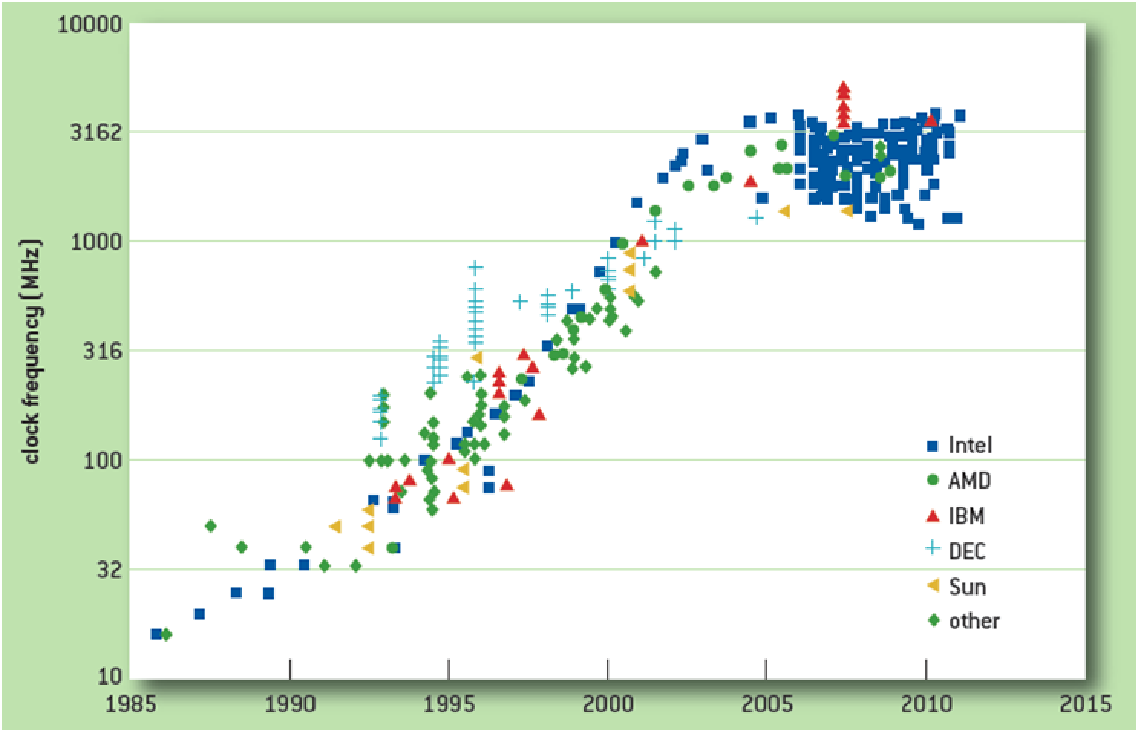
\includegraphics[width=0.6\linewidth]{chap1fig/cpuscaling.pdf}
\caption{Processor Frequency Scaling Over Time~\cite{Danowitz:2012:CDR:2133806.2133822}
\label{fig:cpuscaling}}
\end{center}
\end{figure}

During the rise of 
parallel computer systems, the research community created many auto parallelization tools~\cite{Wilson:1994:SCS:891422}~\cite{Blume94polaris:the}~\cite{oscar},
to relieve the programmers from the tedious manual parallelization process. As real applications
often contain irregular algorithms which are hard to analyze, various
mechanisms were also proposed for users to provide hints/interactively guide the parallelizing compiler~\cite{RiceUniversity:1993:HPF:174223.158909}~\cite{Liao:1999:SEI:329366.301108}~\cite{86108}.
% 
A very similar trend, is currently happening in the heterogeneous computing realm as well.



\section{Heterogeneous Computing with Field Programmable Gate Arrays}
\label{chap1:het}
Field programmable gate array (FPGA) is a fundamentally different computation device
compared to the conventional microprocessors. Figure~\ref{fig:fpgaArch}
shows a simple FPGA which contains a matrix
of logic blocks connected by programmable interconnect. Each logic block
can be configured to perform different compute operations while the interconnect links them together to form a fixed function hardware engine.
Compare to application specific integrated circuits(ASICs), the FPGA configurations can be easily changed to implement many different functions,
accommodating various needs of the users.
This flexibility of course comes at a cost. As the logic and
routing resources are all reprogrammable mechanisms supported by RAM bits, there are significant
area, performance and power overheads compared to the ASICs~\cite{4068926}. To alleviate these disadvantages, 
more specialized circuits like block RAM and DSP blocks are added to modern
FPGAs~\cite{chips:virtex5}~\cite{chips:arria}. Subsequently some of the common functionalities can be mapped onto
these blocks and get closer to ASIC performance/power. When an application
is implemented on an FPGA, arithmetic and logic operations are spatially mapped to
the various compute resources in the reconfigurable array, while the dependencies between them
are satisfied by physical connections formed with on-chip routing resources. Compare to the CPUs, where the ALUs are heavily time
multiplexed, FPGAs can perform orders of magnitude more operations every clock cycle due to its
massive parallelism. For the right kind of computation, FPGAs offer an attractive
trade-off between flexibility and efficiency compared to ASICs and CPUs, and
thus occupy a unique space in the spectrum of computing devices.

%The actual performance achievable certainly depends 
%on the nature of the application. Inherently serial functions may not be
%able to make use of abundance of computing resources and can have better
%speed on CPUs, due to the high clock frequency.


\begin{figure}[htp]
\begin{center}
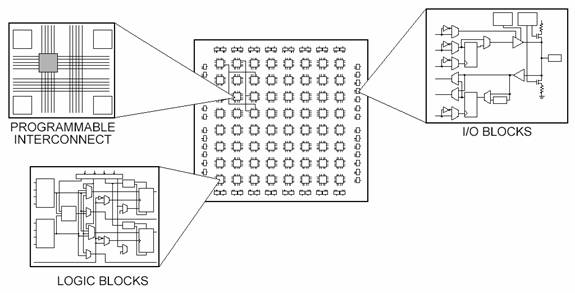
\includegraphics[width=0.8\linewidth]{chap1fig/archsim.jpg}
\caption{Simplified FPGA Architecture~\cite{fpgafun}
\label{fig:fpgaArch}}
\end{center}
\end{figure}

When CPUs are combined with FPGAs,
the resulted heterogeneous platforms would allow the users to place workloads onto the most appropriate
computing device to increase overall system efficiency.
Inherently serial functions may not be able to make use of the FPGAs' abundance of computing resources and can have better speed on the CPUs, due to its high clock frequency.
Meanwhile, functions with plenty of parallelism can take advantage of the
spatial computing paradigm provided by the FPGAs.
Application specific accelerators implementing these functions can offer
%with their tremendous flexibility, can be configured into application-specific
%accelerators which offer 
huge performance and energy advantages over general purpose
processors. There are many systems where FPGAs are coupled to CPUs through PCIe interconnect, Front Side Bus etc.~\cite{nallatech510T}~\cite{maxeler},
used in application domains ranging from scientific computing, gas and oil exploration to financial analytics
~\cite{smith2005scientific}~\cite{5719584}~\cite{6299067}.
Also, recent developments in FPGA SoCs, where the reconfigurable arrays are  integrated with hard processors and memory interface IPs at the chip level,
have created some highly compact yet versatile computing platforms~\cite{chips:zynq}~\cite{chips:cyclonesoc}. 
However, to make these platforms easily accessible to the application developers, there are still many challenges,
as the programming methodology for FPGAs is rather different than that for the general purpose processors.

%When applications are implemented on FPGAs, arithmetic and logic operations are spatially mapped to
%the various compute resources in the reconfigurable array, while the dependencies between them
%are satisfied by physical connections formed with on-chip routing resources. %Compare to the CPUs, where the ALUs are heavily time
%multiplexed, FPGAs can perform orders of magnitude more operations every clock cyle due to its
%massive parallelism. 
Traditionally, FPGAs are programmed using register transfer level (RTL) design
abstraction. The designers not only have to extract both coarse-grain and fine-grain parallelism in the
application, but also
need to define the behavior of the final implementation down to every clock cycle.
Hardware design principles such as clock management, state machines,
pipelining, and device specific memory management must be employed to really unlock the potential
in FPGA computing. All these concepts are unfortunately outside the expertise of most application-oriented
software developers. 

\section{High Level Synthesis} 
\label{chap1:hls}
Given the difficulty in progamming FPGAs, there has
been a trend towards design synthesis from higher levels of
specifications~\cite{Coussy:2008:HSA:1457713},~\cite{intro2hls}. Being more compact and expressive, high level
languages, when used as design input, can greatly increase the
productivity of engineers. Just like in the case of parallelizing compilers, the gap between
an efficient implementation and a productive programming experience attracted major interest from 
both industry and academia. Many commercial,~\cite{tools:autoesl},~\cite{tools:catapultc}~\cite{tools:alterac2h},~\cite{tools:vivadohls} and open source~\cite{tools:legup},~\cite{tools:roccc} tools have been developed over the years 
to tackle this challenge of generating hardware functional blocks from high level
behavioral descriptions. Programming languages such as C/C++, designed for processor-centric execution, are used by these high-level synthesis programs as the medium for input specification. 

All these HLS tools attempt to capture parallelism in the control dataflow described by high level languages, often with various forms of guidance provided by the user, and 
generate hardware in the form of RTL.
Compute operations and memory accesses are allocated and scheduled according to the dependency constraints extracted
from analysis and resource constraints imposed by the target platform. The circuits generated usually follow
a Finite State Machine with Datapath (FSMD) paradigm. Activation of a particular operator in the datapath is associated
with a certain clock cycle and the execution of the entire control dataflow graph is orchestrated by 
a synthesized central controller. Depending on the system architecture, the generated hardware can have
different mechanisms in accessing the memory.
In some systems, direct memory access(DMA) engines are instantiated and data movements are explicitly managed, while 
%In the context of a CPU+accelerator system, 
in others, the generated
hardware is presented with a memory interface rather similar to that used by a processor, with various
caching schemes~\cite{6239785}~\cite{6239808} proposed to complement the datapath.

With the HLS tools, it seems the programmers now have an easy path to offloading the compute intensive parts of their software
to FPGAs, but the performance boost and energy efficiency of the mapped implementations are
often less than ideal. 
%The barrier between software and the reconfigurable fabric is more than just the language used, the
%difference in the paradigms of computation would also need to be addressed.
%This combination of new tools and devices has created new opportunities for applications written in high level languages.  
%Applications can be mapped to these heterogeneous 
%substrates, with the compute intensive loop nests running in accelerators and the remainder of the 
%code executing on processors.
%However, the performance boost and energy efficiency of the mapped implementations are
%often less than optimal
%when HLS tools are employed to directly map the software code to the reconfigurable fabric.
%%The application kernels, originally written for processor execution, may not be amenable for hardware implementation. 
%The barrier between software and the FPGA fabric is
%more than just the programming language used---real difference lies
%in the paradigms of computation.
%To produce good FPGA designs with HLS, 
%the users still have to visualize and create hardware descriptions,
%albeit with the C/C++ syntax.
%To effectively harness the power of reconfigurable platforms for software acceleration, designers usually need to identify parallelism
%in the application, which can then be exploited by the tool with the addition of pragmas and directives. 
%More often than not, the hardware infrastrucutre for data movement into and out of on chip buffers also need to be created and managed explicitly.
%In most scenarios, there is still a trade-off between ease of use and the achieved quality of results.
%In this dissertation, we explore a few approaches in reducing the user effort while producing high performance CPU+accelerators using high level synthesis (HLS).
%\begin{itemize}
%    \item Automatic refactoring of computation kernals into pipelines with decoupled memory access. 
%		FPGA is especially efficient in implementing streaming applications where data move through
%		a cascade of pipeline stages. 
%Also, to boost
%FPGA accelerator efficiency it is often desirable to convert
%from conventional memory accesses to a streaming model
%and to insert DMA engines [6]. Further enhancements can be
%achieved by including accelerator specific caching and burst
%accesses.
%    \item automatic tuning of processing pipeline using runtime profile
%    \item generation and integration of accelerator from program binary for regular computation kernels 
%\end{itemize}
To produce good FPGA designs with HLS, 
the users still have to visualize and create hardware descriptions,
albeit with the C/C++ syntax.
To effectively harness the power of reconfigurable platforms for software acceleration, designers usually need to identify parallelism
in the application, which can then be exploited by the tool with the addition of pragmas and directives. 
More often than not, the hardware infrastrucutre for data movement into and out of on chip buffers also need to be created and managed explicitly.
In most scenarios, there is still a trade-off between ease of use and the achieved quality of results. 
It is thus important to provide methods in parallelism discovery, design space exploration and system integration
to help the user better take advantage of this unique compute substrate.
\section{Dissertation Organization}

In this dissertation, we present tools and mechanisms for optimizing, analyzing and integrating HLS generated accelerators.
%and easing the integration of them into applications. 

\subsection{Synthesis of computational pipelines with decoupled memory access}

The first flow we created transforms a sequential program into a computational pipeline consisted of multiple
processing stages connected by communication channels. FPGA is especially efficient in implementing streaming 
applications where data move through a cascade of pipeline stages. This is unfortunately not how a typical 
C/C++ program describes its computation. By utilizing pipeline parallelism in sequential programs, 
%we can drastically improve the performance of generated
%accelerator.
we generate elastic pipelines with much better tolerance towards data access latency.
For programs with memory footprint greater than the on-chip RAM capacity, significant improvement in performance
can be achieved. Within the same framework, conventional memory accesses are converted to a streaming model whenever
possible, with customized caching and burst accesses to further boost the accelerator efficiency. 
In chapter~\ref{decoupleChap}, the implementation details of this flow are presented. To demonstrate 
the advantage of our approach, experimental results comparing it against state-of-the-art HLS tools
are also presented.

\subsection{Deadlock prevention in network of statically scheduled accelerators}
In synthesizing the decoupled computational pipeline, the original program
is essentially converted to a network of processes, each executed by a statically scheduled accelerator. In chapter~\ref{liveprof}, we create a framework to analyze the property of this network, leveraging past research in Kahn process networks, to determine conditions for liveness of our generated pipeline. 
Contrary to past simulation-based approach, we examine the interaction between the static scheduling by HLS and the sizing of the communication channels between the processes to find ways to prevent deadlock \textit{a priori}. We also
discuss how our technique may be used in other more generalized context.
\begin{comment}
With the communication channels being fixed in size, 

As each of these processes is eventually implemented using HLS, its schedule is statically generated. We generalize our approach to 
As communication
channels are implemented using FIFOs in the FPGA, the buffer space in our pipelines is always bounded. 
A natural concern is the liveness of the pipeline. This is addressed with a formal proof in chapter~\ref{liveprof}.
\end{comment}

\begin{comment}

\subsection{Tuning of processing pipeline using runtime profile}
When the generated pipeline stages contain data-dependent control flow and memory access patterns, 
it becomes difficult to optimize as the program behavior cannot be analyzed statically. 
%To guide the design space exploration, runtime behavior of the pipeline is captured and analyzed. The design can then
%evolve accordingly, taking advantage of the reconfigurability of FPGAs.
The runtime behavior of the pipeline must be captured and examined to identify the performance bottleneck and
guide the design space exploration. More specifically,
%Given the data-dependent nature of control flows in applications and thus in the generated processing stages,
%it is hard to statically analyze and identify performance bottle neck in the computation pipeline. 
by observing the distribution of occupancy of the communication channels over time, we can infer how heavily loaded
each part of our pipeline is. More hardware may be dedicated to heavily loaded processing stages for more aggressive 
parallelization/better caching. The design is therefore evolving according the the characteristics of the
load, taking advantage of the reconfigurability of FPGAs. Chapter~\ref{profileChap} describes the infrastructure for this automatic tuning
of the pipeline based on its runtime behavior. Improvement on quality of results is also shown at the end
of the chapter.
\end{comment}

\subsection{Accelerator generation and integration using program binaries}
To push the limit in usability of FPGA platforms, we explored the generation and 
integration of accelerators with just program binaries. 
%It makes the FPGA completely 
%transparent to the user and can be used even in the absence of source code. 
%Of course, the scope of applications this approach can be applied to is relatively narrow. Only regular computation kernels can be converted to FPGA accelerators.
This approach is only beneficial for more regular applications,
where the memory access patterns are analyzable and coarse grained paralellism can be extracted.
With program binary analysis and instrumentation, it becomes possible to integrate the FPGA-accelerated parts into the original application
in a user transparent way. Neither recompilation of the original program nor the source code
is required. Performing all the analysis based on program binary does introduce more uncertainty
than a source code based approach. Thus we have devised a two phase mechanism to have parts of the 
analysis done during the runtime to ensure correctness. The details are described
in chapter~\ref{instrumentChap}. 

\subsection{}
\vspace{-30.0pt}
Finally in chapter~\ref{concluChap}, we conclude our dissertation and discuss potential directions for
future studies. 
%\subsection{}
%\vspace{-10pt}
\begin{comment}
In this work, we explore a few approaches in reducing the user effort while producing high performance CPU+accelerators systems using high level synthesis (HLS).
\begin{itemize}
    \item \textit{refactoring of computation kernals into pipelines with decoupled memory access.}
		FPGA is especially efficient in implementing streaming applications where data move through
		a cascade of pipeline stages. This is unfortunately not how a typical C/C++ program describes its computation.
		By utilizing pipeline parallelism in sequential programs, we can drastically improve the performance of generated
		accelerator.

%when possible, which greatly alleviate the sensitivity of the accelerator to memory access latency and provided
%Also, to boost FPGA accelerator efficiency it is often desirable to convert 
%		from conventional memory accesses to a streaming model and to insert DMA engines which can perform
%. Further enhancements can be
%		achieved by including accelerator specific caching and burst accesses.
    \item \textit{Tuning of processing pipeline using runtime profile.} 
	When the generated pipeline stages contain data-dependent control flow and memory access patterns, it becomes hard to optimize as the program behavior cannot be analyzed statically. To guide the design space exploration, runtime behavior of the pipeline is captured and analyzed. The design can then
evolve accordingly, taking advantage of the reconfigurability of FPGAs.

    \item \textit{generation and integration of accelerator from program binary for regular computation kernels.} To push the limit
    in usability of FPGA platforms, we explore the generation and integration of accelerators with only program binaries. It makes the FPGA completely transparent to the user and can be used even in the absence of source code. Of course, the scope of applications this approach can be applied to is relatively narrow. Only regular computation kernels can be converted to FPGA accelerators.
\end{itemize}
\end{comment}


%Despite the 
%absence of a universally accepted programming paradigm/language for the front end, progress was being made
%on multiple fronts. 
%The main steps in HLS, allocation  

%Various heuristics in transforming and scheduling computation graphs were examined 
%to achieve different area/performance trade-off~\cite{TrickeyHFlamel},,,~\cite{1586344},~\cite{31534},~\cite{1270207}.
%As the allocation, scheduling and 


\section{Thesis Contributions}

In summary, the main contributions of my thesis include the following:
\begin{itemize}
    \item Advancing the state of the art for high level synthesis by devising a systematic
    method to generate elastic processing pipeline from sequential programs. The pipeline
    parallelism in the source code is effectively harnessed to create higher performance
    accelerators.
    \item Creating an analysis framework for the generated pipeline, which is formulated as a process network. It is then possible to examine the interaction between scheduling and buffer sizing in this network, allowing detection and resolution of deadlocks statically.
    \item Improving the usability of FPGAs by creating a flow which synthesize
    accelerators from program binaries. Various aspects of integrating the accelerators with the original program are also discussed. It is now possible to offload computation to FPGAs in an user-transparent fashion.
    \item Quantifying the benefits of the proposed flows using off-the-shelf FPGA SoCs. The
    performance and area consumption for the benchmarks are presented. Design space exploration is also performed to demonstrate the trade-off between execution time and resource usage.
    
    
\end{itemize}


\begin{comment}
In this dissertation, we present tools and mechanisms for optimizing, analyzing and integrating HLS generated accelerators.
%and easing the integration of them into applications. 

\subsection{Synthesis of computational pipelines with decoupled memory access}

The first flow we created transforms a sequential program into a computational pipeline consisted of multiple
processing stages connected by communication channels. FPGA is especially efficient in implementing streaming 
applications where data move through a cascade of pipeline stages. This is unfortunately not how a typical 
C/C++ program describes its computation. By utilizing pipeline parallelism in sequential programs, 
%we can drastically improve the performance of generated
%accelerator.
we generate elastic pipelines with much better tolerance towards data access latency.
For programs with memory footprint greater than the on-chip RAM capacity, significant improvement in performance
can be achieved. Within the same framework, conventional memory accesses are converted to a streaming model whenever
possible, with customized caching and burst accesses to further boost the accelerator efficiency. 
In chapter~\ref{decoupleChap}, the implementation details of this flow are presented. To demonstrate 
the advantage of our approach, experimental results comparing it against state-of-the-art HLS tools
are also presented.

\subsection{Deadlock Prevention in Network of Statically Scheduled Processes}
In synthesizing the decoupled computational pipeline, the original program
is essentially converted to a network of processes, executed in a distributed manner. In chapter~\ref{liveprof}, we create a framework to analyze the property of this network, leveraging past research in Kahn process networks, to determine conditions for liveness of our generated pipeline. 
Contrary to past simulation-based approach, we examine the interaction between the static scheduling by HLS and the sizing of the communication channels between the processes to find ways to prevent deadlock \textit{a priori}. We also
discuss how our technique may be used in other more generalized context.
\end{comment}




\begin{comment}
With the communication channels being fixed in size, 

As each of these processes is eventually implemented using HLS, its schedule is statically generated. We generalize our approach to 
As communication
channels are implemented using FIFOs in the FPGA, the buffer space in our pipelines is always bounded. 
A natural concern is the liveness of the pipeline. This is addressed with a formal proof in chapter~\ref{liveprof}.
\end{comment}

\begin{comment}

\subsection{Tuning of processing pipeline using runtime profile}
When the generated pipeline stages contain data-dependent control flow and memory access patterns, 
it becomes difficult to optimize as the program behavior cannot be analyzed statically. 
%To guide the design space exploration, runtime behavior of the pipeline is captured and analyzed. The design can then
%evolve accordingly, taking advantage of the reconfigurability of FPGAs.
The runtime behavior of the pipeline must be captured and examined to identify the performance bottleneck and
guide the design space exploration. More specifically,
%Given the data-dependent nature of control flows in applications and thus in the generated processing stages,
%it is hard to statically analyze and identify performance bottle neck in the computation pipeline. 
by observing the distribution of occupancy of the communication channels over time, we can infer how heavily loaded
each part of our pipeline is. More hardware may be dedicated to heavily loaded processing stages for more aggressive 
parallelization/better caching. The design is therefore evolving according the the characteristics of the
load, taking advantage of the reconfigurability of FPGAs. Chapter~\ref{profileChap} describes the infrastructure for this automatic tuning
of the pipeline based on its runtime behavior. Improvement on quality of results is also shown at the end
of the chapter.
\end{comment}


\begin{comment}
\subsection{Accelerator generation and integration using program binaries}
To push the limit in usability of FPGA platforms, we explored the generation and 
integration of accelerators with only program binaries. 
%It makes the FPGA completely 
%transparent to the user and can be used even in the absence of source code. 
%Of course, the scope of applications this approach can be applied to is relatively narrow. Only regular computation kernels can be converted to FPGA accelerators.
This approach is only beneficial for more regular applications,
where the memory access patterns are analyzable and coarse grained paralellism can be extracted.
With program binary analysis and instrumentation, we can have the FPGA-accelerated parts of the application
integrated in a user transparent way. Neither recompilation of the original program nor the source code
is required. Performing all the analysis based on program binary does introduce more uncertainty
than a source code based approach. Thus we have devised a two phase mechanism to have parts of the 
analysis done during the runtime to ensure correctness. The details are described
in chapter~\ref{instrumentChap}. 

\subsection{}
\vspace{-30.0pt}
Finally in chapter~\ref{concluChap}, we conclude our research and discuss potential directions for
future studies. 
\end{comment}
%\begin{itemize}
 %   \item \textit{Automatic refactoring of computation kernals into pipelines with decoupled memory access.}
%		FPGA is especially efficient in implementing streaming applications where data move through
%		a cascade of pipeline stages. A flow was developed to create this pipeline from a sequential program.
%The flow also converts conventional memory accesses to a streaming model, with customized caching and burst accesses
%to further boost the accelerator efficiency.
%when possible, which greatly alleviate the sensitivity of the accelerator to memory access latency and provided
%Also, to boost FPGA accelerator efficiency it is often desirable to convert 
%		from conventional memory accesses to a streaming model and to insert DMA engines which can perform
%. Further enhancements can be
%		achieved by including accelerator specific caching and burst accesses.
%    \item \textit{automatic tuning of processing pipeline using runtime profile.} When the generated pipeline stages contain data-dependent control flow and memory access patterns, it becomes hard to optimize as the program behavior cannot be analyzed statically.
%    However, by observing the runtime occupancy of the communication channels in the pipeline, we can identify the bottlenecks and
%    tune the structure of the processing pipeline, taking advantage of the reconfigurability of FPGAs.
%    \item \textit{generation and integration of accelerator from program binary for regular computation kernels.} To push the limit
%    in usability of FPGA platforms, we explore the generation and integration of accelerators with only program binaries. It makes the FPGA completely transparent to the user and can be used even in the absence of source code. Of course, the scope of applications this approach can be applied to is relatively narrow. Only regular computation kernels are converted to FPGA accelerators.
 %   \end{itemize}

%designers often need to restructure the original code to separate out memory 
%accesses before invoking HLS.
%Also, to boost FPGA accelerator efficiecy it is desireable to convert 
%from conventional memory accesses to a streaming model and to insert DMA engines~\cite{vivado_hls:appnoteMMult}.   Further enhancements can be achieved by incuding 
%accelerator specific caching and burst accesses.

%for scheduling of operations in 
%data-flow designs. Simple methods were proposed where operations are scheduled as early
%as possible (ASAP) or as late as possible (ALAP)


